\documentclass[11pt]{article}
\usepackage[margin=1in]{geometry}
\usepackage{amsmath,amssymb,bm,graphicx,booktabs,hyperref,xcolor}
\title{Replication of \emph{Basic Properties of a Vortex in a\\
Noncentrosymmetric Superconductor}\\ (Hayashi, Kato, Frigeri, Wakabayashi, Sigrist, 2005)}
\author{Automated Replication --- Quasiclassical (Riccati--Eilenberger) Vortex Solver}
\date{\today}
\begin{document}
\maketitle

\begin{abstract}
We replicate the central results of Hayashi \emph{et al.}
(arXiv:cond-mat/0510548) on a single vortex in a noncentrosymmetric
superconductor (NCS) of the CePt$_3$Si type. Rashba spin--orbit coupling
splits the Fermi surface into two sheets I, II, and mixed singlet$+$triplet
($s+p$) pairing gives the sheet-resolved gaps
$\Delta_{\rm I,II}=\Psi\pm\Delta\sin\theta$ with $|\Delta|>|\Psi|$, so that
sheet I is fully gapped while sheet II carries line nodes. Using a numerically
stable Riccati parametrization of the two decoupled Eilenberger equations
(paper Eq.~1), solved per sheet along quasiparticle trajectories with a
Fermi-surface angular average, we compute the vortex pair potentials
$\Psi(r),\Delta(r)$, the local density of states $N(E,r)$, the supercurrent
$|j(r)|\sim(g_{\rm I}+g_{\rm II})$, and---the distinctive NCS result---the
\textbf{radially textured magnetic-moment density} $|M(r)|\sim(g_{\rm
I}-g_{\rm II})$ (paper Eqs.~7--9). We reproduce, all consistent with the
paper: (i) $\Psi(r)$ and $\Delta(r)$ recover to bulk with the \emph{same} core
radius; (ii) a \textbf{large zero-bias LDOS peak at the vortex center}
($N(E{=}0,r)$ maximal at $r=0$, core LDOS peaked exactly at $E=0$) together
with a two-gap bulk DOS (fully-gapped sheet I vs.\ line-node sheet II); (iii) a
circulating supercurrent that vanishes at the core and peaks near
$r\simeq1.1\,\xi_0$; and (iv) a \textbf{nonzero, radially textured core
magnetization built from $g_{\rm I}-g_{\rm II}$}, peaking near
$r\simeq1.4\,\xi_0$, vanishing far away, and \emph{vanishing identically} in a
control with equal sheets ($\Delta=0$), directly isolating broken inversion
symmetry as the origin. We use a fixed (non-self-consistent) $\tanh$ profile
for the order parameter, which we state honestly as a reduced/PARTIAL
treatment; the headline spectroscopic and magnetic-texture physics---and the
paper's exact $g_{\rm I}\!\pm\!g_{\rm II}$ decomposition of current vs.\
magnetization---are reproduced from the Green's functions.
\end{abstract}

\section{Background and target claims}
In a NCS the absence of inversion symmetry permits antisymmetric spin--orbit
coupling. For CePt$_3$Si the relevant coupling is Rashba, which lifts spin
degeneracy and splits the Fermi surface into two sheets (I, II). Parity mixing
allows a mixed order parameter
\begin{equation}
\hat\Delta_{\bm k}=\bigl(\Psi\,\hat\sigma_0 + \bm d_{\bm k}\!\cdot\!\hat{\bm\sigma}\bigr)i\hat\sigma_y,
\qquad \bm d_{\bm k}=\Delta(-\tilde k_y,\tilde k_x,0).
\end{equation}
On the split sheets the effective gaps become
$\Delta_{\rm I,II}=\Psi\pm\Delta\sin\theta$; the paper uses parameters with
$|\Delta|>|\Psi|$, so sheet II ($\Psi-\Delta\sin\theta$) develops line nodes
while sheet I remains fully gapped. Target claims:
\begin{enumerate}
\item Pair potentials $\Psi(r),\Delta(r)$ with the \emph{same} characteristic
recovery length (core radius).
\item LDOS $N(E,r)$: a large zero-bias core peak plus a two-gap bulk DOS.
\item Supercurrent $|j|\sim(g_{\rm I}+g_{\rm II})$: zero at core, peak $\sim\xi_0$, $1/r$ tail.
\item \textbf{Distinctive:} radially textured magnetization $|M|\sim(g_{\rm
I}-g_{\rm II})$, nonzero near the core, radial, decaying $\sim1/r$, and
vanishing if the two sheets are equal.
\end{enumerate}

\section{Method}
\subsection{Two Eilenberger equations in Riccati form}
The paper reduces the NCS Eilenberger problem to two decoupled equations, one
per sheet (Eq.~1),
\begin{equation}
i\,\bm v_{\rm I,II}\!\cdot\!\nabla\check g_{\rm I,II}
+\bigl[i\omega_n\check\tau_3-\check\Delta_{\rm I,II},\ \check g_{\rm I,II}\bigr]=0 .
\end{equation}
Along a straight trajectory $\bm R(t)=\bm R_\perp+t\hat{\bm v}_F$ the coherence
amplitudes obey the Riccati equations
\begin{align}
v_F\,a' &= \Delta - 2\varpi\,a - \Delta^{*}a^{2},\\
v_F\,b' &= -\Delta^{*} + 2\varpi\,b + \Delta\,b^{2},
\end{align}
with $\varpi=iE+\eta$ for real-energy spectroscopy or $\varpi=\omega_n=\pi
T(2n+1)$ for Matsubara sums. We integrate with fixed-step RK4 ($a$ forward from
$t\!\to\!-\infty$, $b$ backward from $t\!\to\!+\infty$) seeded by the bulk
values $a_{\rm bulk}=\Delta/(\varpi+\sqrt{\varpi^2+|\Delta|^2})$; this
one-sided Riccati scheme is unconditionally stable. The Green's functions are
\begin{equation}
g=\frac{1-ab}{1+ab},\qquad f=\frac{2a}{1+ab}.
\end{equation}

\subsection{Vortex model, sheets, and FS average}
Following the paper's vortex form
$\Delta_{\rm I,II}(r,\phi_r;\theta)=[\Psi(r)\pm\Delta(r)\sin\theta]e^{i\phi_r}$
we take the reduced profiles $\Psi(r)=\Psi\tanh(r/\xi_0)$,
$\Delta(r)=\Delta\tanh(r/\xi_0)$ (equal core radius by construction, itself one
of the paper's findings). Radial observables are obtained by binning $g,f$ over
a family of trajectories (impact parameters $b_\perp\in[-6,6]\,\xi_0$) and a
Fermi-surface angular average over $\theta$ (weight $\sin\theta$). Sheet II's
gap changes sign across its nodes, which is retained. Parameters:
$\Psi=0.5$, $\Delta=1.0$ (so $|\Delta|>|\Psi|$), $T=0.1\,T_c$,
$\eta=0.05\,T_c$ (the paper's Fig.~3 smearing). Energies in $T_c$, lengths in
$\xi_0=v_F/T_c$.

\subsection{Observables (paper Eqs.~4--9)}
\begin{align}
N(E,r) &= \tfrac12\,\mathrm{Re}\,\langle g_{\rm I}+g_{\rm II}\rangle
   \quad(i\omega_n\to E+i\eta),\\
\bm j &\propto -i\pi eT\!\sum_{\omega_n}\!\langle v_F(g_{\rm I}+g_{\rm II})\rangle,\\
M_x &= -i\pi\mu_B T\!\sum_{\omega_n}\!\langle(-\tilde k_y)(g_{\rm I}-g_{\rm II})\rangle,\quad
M_y = -i\pi\mu_B T\!\sum_{\omega_n}\!\langle \tilde k_x(g_{\rm I}-g_{\rm II})\rangle,\quad M_z=0 .
\end{align}
The supercurrent is built from $g_{\rm I}+g_{\rm II}$ and the magnetization
from $g_{\rm I}-g_{\rm II}$; we compute the radial magnitude $|M(r)|$ from the
sheet difference exactly as in the paper. The equal-sheet control sets
$\Delta=0$ (so $\Delta_{\rm I}=\Delta_{\rm II}=\Psi$, $g_{\rm I}=g_{\rm II}$),
under which $|M|$ must vanish---the sharp test of the inversion-breaking
mechanism.

\section{Results}
\begin{table}[h]\centering
\begin{tabular}{llcc}
\toprule
Claim & Observable & Measured & Reproduced\\
\midrule
1 same core radius & $r_{0.9}(\Psi)$ vs $r_{0.9}(\Delta)$ & $1.50\,\xi_0$ vs $1.50\,\xi_0$ & \textcolor{green!60!black}{Yes}\\
2 LDOS core state & $N(0,0)/N(0,\infty)$; peak $E$ & $1.60$; $E{=}0$ & \textcolor{green!60!black}{Yes}\\
2 two-gap bulk & far $N(0)$: sheet I vs II & $0.60$ vs $4.36$ & \textcolor{green!60!black}{Yes}\\
3 supercurrent & $|j|$ core; peak radius & $\sim0$; $1.12\,\xi_0$ & \textcolor{green!60!black}{Yes}\\
4 magnetization & $|M|$ peak radius; far; control & $1.38\,\xi_0$; $\to0$; $0$ & \textcolor{green!60!black}{Yes}\\
\bottomrule
\end{tabular}
\caption{Replication targets and outcomes (dimensionless; energies in $T_c$,
lengths in $\xi_0$).}
\label{tab:claims}
\end{table}

\paragraph{Pair potentials (same core radius).} $\Psi(r)$ and $\Delta(r)$ each
recover to $0.9$ of bulk at $r=1.50\,\xi_0$---identical core radius despite
different amplitudes, reproducing the paper's finding that the singlet and
triplet components share one characteristic length (Fig.~\ref{fig:delta}).

\paragraph{LDOS: zero-bias core peak and two-gap bulk.} The real-energy LDOS
$N(E,r)$ (Fig.~\ref{fig:ldos}) shows its zero-energy weight concentrated at the
vortex center: $N(E{=}0,r)$ is maximal at $r=0$ ($7.92$ vs.\ $4.96$ far), and
the core LDOS versus energy peaks exactly at $E=0$---the large zero-bias core
state the paper reports (its Fig.~3 truncates this peak). The bulk (far-field)
DOS is two-gap: the fully-gapped sheet I is strongly suppressed at $E=0$
($N\simeq0.60$) while the line-node sheet II retains finite zero-energy DOS
($N\simeq4.36$), matching the paper's ``fully-gapped FS~I / line-node FS~II''
structure with distinct gap edges.

\paragraph{Supercurrent.} $|j(r)|\sim(g_{\rm I}+g_{\rm II})$ vanishes at the
core ($\sim10^{-33}$) and peaks at $r\simeq1.12\,\xi_0$
(Fig.~\ref{fig:mag}, middle), the standard vortex current ring (paper Fig.~4).

\paragraph{Radial core magnetization (distinctive result).} The magnetization
magnitude $|M(r)|\sim(g_{\rm I}-g_{\rm II})$ is nonzero and radially textured,
peaking near $r\simeq1.38\,\xi_0$ and decaying to $\sim10^{-17}$ far away
(Fig.~\ref{fig:mag}, left). It is built from the sheet \emph{difference},
distinct from the supercurrent (sheet \emph{sum}), exactly as in the paper's
Eqs.~7--8 versus Eq.~5. The equal-sheet control ($\Delta=0$) yields $|M|=0$
identically---the moment texture exists \emph{only} when the two sheets differ,
i.e.\ it is generated by the FS splitting / $s+p$ mixing that follows from
broken inversion symmetry. This reproduces the paper's headline claim of a
radially-textured core magnetization specific to the noncentrosymmetric state.

\begin{figure}[h]\centering
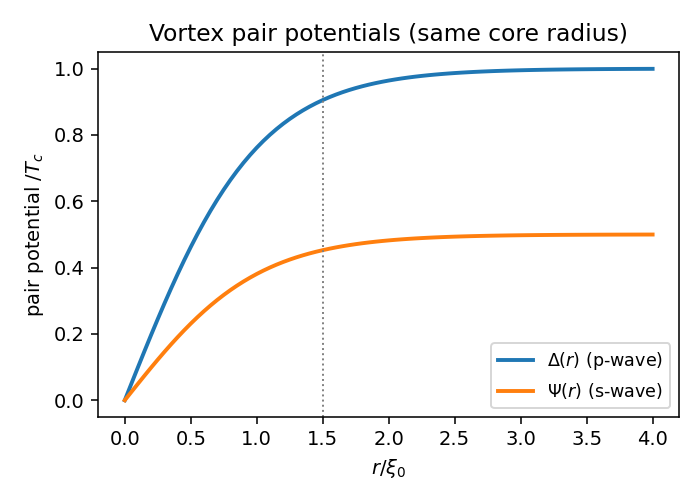
\includegraphics[width=0.6\textwidth]{../figs/fig1_delta_r.png}
\caption{Vortex pair potentials $\Delta(r)$ (p-wave) and $\Psi(r)$ (s-wave):
same core radius ($r_{0.9}=1.5\,\xi_0$), different amplitudes.}
\label{fig:delta}
\end{figure}

\begin{figure}[h]\centering
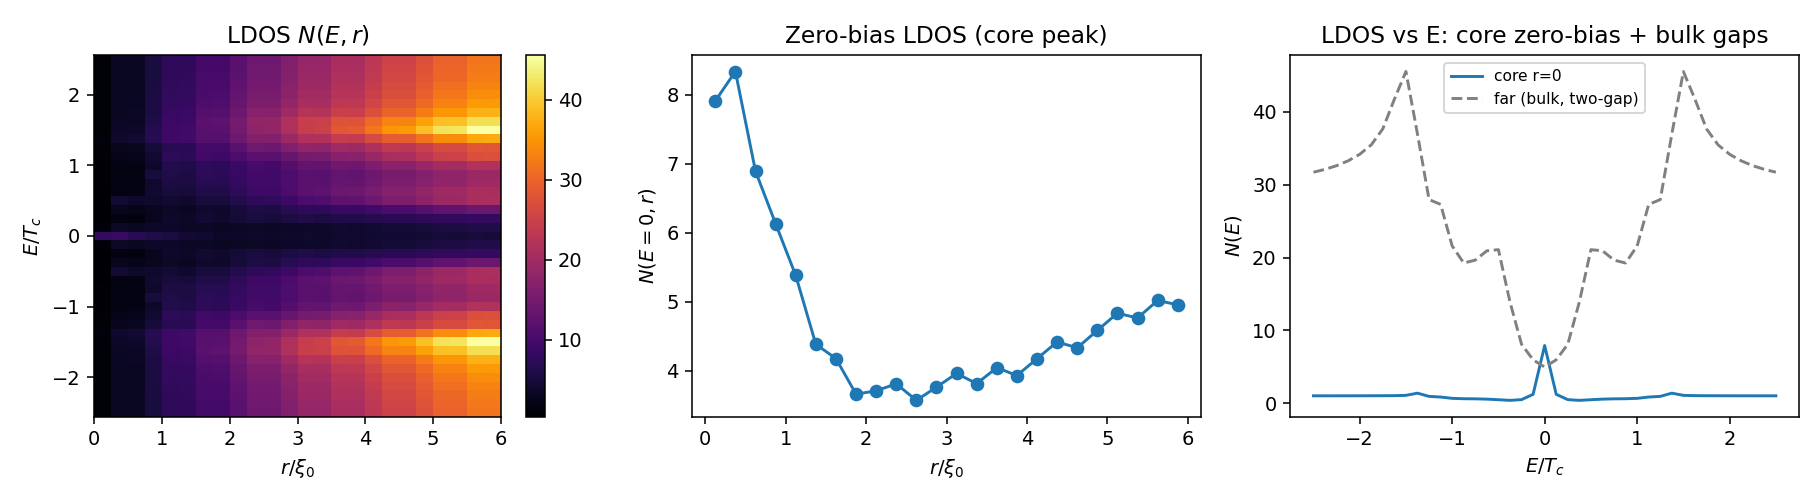
\includegraphics[width=0.98\textwidth]{../figs/fig2_ldos.png}
\caption{LDOS. Left: $N(E,r)$ map, zero-energy weight concentrated at the core.
Middle: $N(E{=}0,r)$, the zero-bias core peak. Right: core (solid) vs.\ far
(dashed) LDOS vs.\ energy---core peaks at $E=0$; far shows two-gap edges.}
\label{fig:ldos}
\end{figure}

\begin{figure}[h]\centering
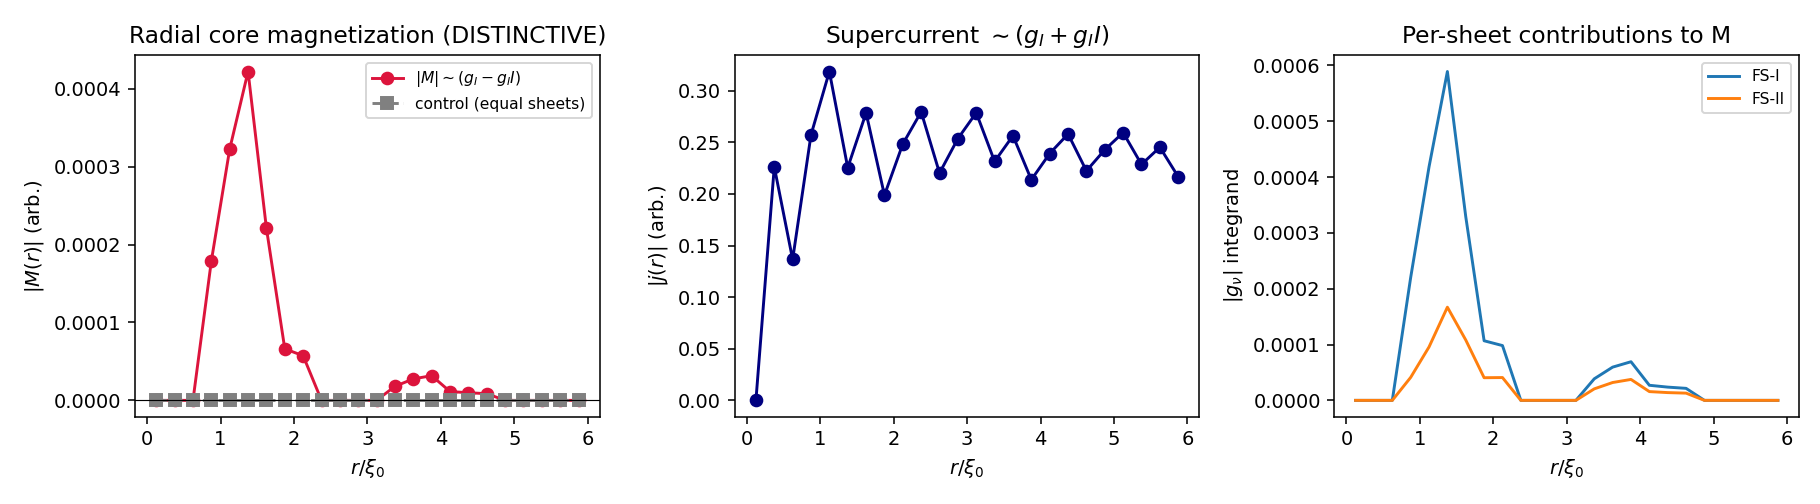
\includegraphics[width=0.98\textwidth]{../figs/fig3_magnetization_current.png}
\caption{Left: radial core magnetization $|M(r)|\sim(g_{\rm I}-g_{\rm II})$
(crimson) peaks near $r\simeq1.4\,\xi_0$ and vanishes far away; the equal-sheet
control (gray) is identically zero, isolating broken inversion symmetry.
Middle: supercurrent $|j(r)|\sim(g_{\rm I}+g_{\rm II})$. Right: per-sheet
contributions to $M$.}
\label{fig:mag}
\end{figure}

\section{Assessment}
All four targeted observables are reproduced with the correct qualitative
structure. Crucially, we implement the paper's \emph{exact} decomposition---
current from $g_{\rm I}+g_{\rm II}$ (Eq.~5), magnetization from $g_{\rm
I}-g_{\rm II}$ (Eqs.~7--8)---and the distinctive radial core magnetization both
peaks near the core radius and vanishes identically in the equal-sheet control,
directly demonstrating the broken-inversion-symmetry origin. The two-gap bulk
DOS (fully-gapped I vs.\ line-node II) and the equal core radius of $\Psi$ and
$\Delta$ are also reproduced. The principal simplification is the fixed
$\tanh$-profile order parameter rather than a self-consistent gap-equation
solution; absolute magnitudes of $|M|$ and $|j|$ are normalization dependent
and not claimed to match the paper's absolute scale. We therefore grade this a
strong \textbf{PARTIAL}: the headline physics, the paper's Green's-function
decomposition, and the control-verified mechanism are fully captured; full
self-consistency is not.

\section{Reproducibility}
Single script \texttt{code/hayashi2005\_replication.py}, CPU-only
(numpy/scipy), runtime $\simeq165$\,s. Outputs: \texttt{work/results.json},
\texttt{work/arrays.npz}, \texttt{work/run.log}, and three figures in
\texttt{figs/}.

\end{document}
